\documentclass[screen, aspectratio=169]{beamer}
\usepackage[T1]{fontenc}
\usepackage[utf8]{inputenc}

% Use the NTNU-temaet for beamer 
% \usetheme[style=ntnu|simple|vertical|horizontal, 
%     language=bm|nn|en, 
%     smalltitle, 
%     city=all|trondheim|alesund|gjovik]{ntnu2017}
\usetheme[style=ntnu,language=en]{ntnu2017}

\usepackage[english]{babel}
\usepackage[style=numeric,backend=biber,natbib=false,sorting=none]{biblatex}

\title[HCI-intro]{Human Computer Interaction}
\subtitle{Introduction}
\author[A. Xamb{\'o}]{Anna Xamb{\'o}}
\institute[NTNU]{Department of Music, NTNU}
\date{October 22, 2019}
%\date{} % To have an empty date

\addbibresource{../hci-lectures.bib} % Add bibliography database

% Set the reference style to numeric.
% See here: http://tex.stackexchange.com/questions/68080/beamer-bibliography-icon
\setbeamertemplate{bibliography item}[text] 

% Set bibliography fonts to a small size.
\renewcommand*{\bibfont}{\footnotesize}

\begin{document}

\begin{frame}
  \titlepage
\end{frame}

% Alternatively, special title page command to get a different background
% \ntnutitlepage

\begin{frame}
\frametitle{Course Design Criteria}
\begin{itemize}
\item Facilitate a lively discussion about the discipline of HCI with particular focus on NIMEs.
\item Explore individually and in group the fundamental concepts behind HCI applied to the work produced during the physical computing workshop.
\item Promote the language used in research (e.g. oral presentations and paper writing).
\item Contextualize the seminar lectures to the broader context of HCI and interactive systems for music performance at a theoretical level (e.g. readings).
\end{itemize}
\end{frame}
%
\begin{frame}
\frametitle{What are the Lectures About?}
\begin{itemize}
\item A 4-lecture series about the theory and practice in the field of human-computer interaction applied to music technology.
\item First two sessions: Broader perspective of HCI (trends and research methods).
\item Last two sessions: Focus on the NIME community (practices, instrument design).
\item Readings are expected before coming to class and the class will be used to discuss the topics in a paced manner.
\item These discussions should be helpful for the final assignment: write a short paper about the system that you have developed in the physical computing workshop.
\end{itemize}
\end{frame}
%
\begin{frame}
\frametitle{Outline}
\begin{itemize}
\item 1st day: Trends in HCI.
\item 2nd day: Evaluation in HCI.
\item 3rd day: NIMEs (focusing on practice).
\item 4th day: NIMEs (focusing on instrument design).
\end{itemize}
\end{frame}
%
\begin{frame}
\frametitle{General Learning Outcomes}
\begin{itemize}
\item Develop critical thinking skills applied to HCI and NIME research.
\item Explore how to do research and write about a self-built prototype of an interactive system for music performance.
\item Discover new trends in the HCI and NIME disciplines.
\item Discuss a diversity range of practices in the HCI and NIME disciplines.
\end{itemize}
\end{frame}
%
\begin{frame}
\frametitle{Grading}
\begin{itemize}
\item 40\% Individual work vs\ 40\% Group work\\
\emph{You need to send individual and group summaries (before and after class respectively) of the suggested readings and participate in the discussions in class to get a positive grade. The final assignment will be writing a paper with individual and group parts.}
\item 40\% Daily work vs\ 40\% Final assignment work\\
\emph{You will be expected to participate both in the daily assignments and in the final assignment to have a positive grade.}
\item 20\% Participatory assistance\\
\emph{An overall participatory attitude and regular assistance can improve the grade.}
\end{itemize}
\end{frame}
%
\begin{frame}
\frametitle{Previous Knowledge / Preparation}
\begin{itemize}
\item Every day you should check the suggested reading(s) that will be discussed at the beginning of the class.
\end{itemize}
\end{frame}
%
\begin{frame}
\frametitle{Recommended General Readings}
\begin{figure}
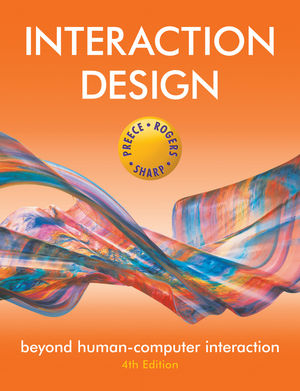
\includegraphics[scale=1]{img/id-book.jpg}
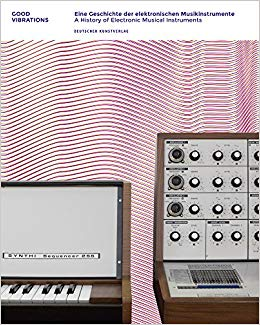
\includegraphics[scale=0.29]{img/good-vibrations-book.jpg}
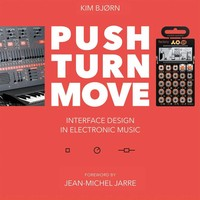
\includegraphics[scale=0.46]{img/push-turn-move-book.jpg}
\end{figure}
\begin{itemize}
\item The book \emph{Interaction Design: Beyond Human-Computer Interaction} by Jenny Preece, Yvonne Rogers and Helen Sharp~\cite{Preece.et.al.2015.ic-book}.
\item The book \emph{New Digital Musical Instruments: Control and Interaction Beyond the Keyboard} by Eduardo Miranda and  Marcelo Wanderley~\cite{Miranda.Wanderley.2006}.
\item The book \emph{Good Vibrations: Eine Geschichte der elektronischen Musikinstrumente / A History of Electronic Musical Instruments}~\cite{Brilmayer.et.al.2018.goodvibrations}.
\item The book \emph{Push Turn Move} by Kim Bj{\o}rn~\cite{Bjorn.2017.pushturnmove}.
\end{itemize}
\end{frame}
%
\begin{frame}
  \frametitle{References}
  \printbibliography
\end{frame}
%
\end{document}
